\documentclass[tikz]{standalone}
\usepackage{cmap}
\usepackage[T2A]{fontenc}
\usepackage[utf8x]{inputenc}
\usepackage{pgfplots}
\usepackage{pgfplotstable,xcolor}
\pgfplotsset{compat=newest}
\usepgfplotslibrary{polar}
\usetikzlibrary{decorations.markings}
\definecolor{color0}{HTML}{e2431e}
\definecolor{color1}{HTML}{e7711b}
\definecolor{color2}{HTML}{f1ca3a}
\definecolor{color3}{HTML}{6f9654}
\definecolor{color4}{HTML}{1c91c0}
\definecolor{color5}{HTML}{43459d}
\begin{document}
	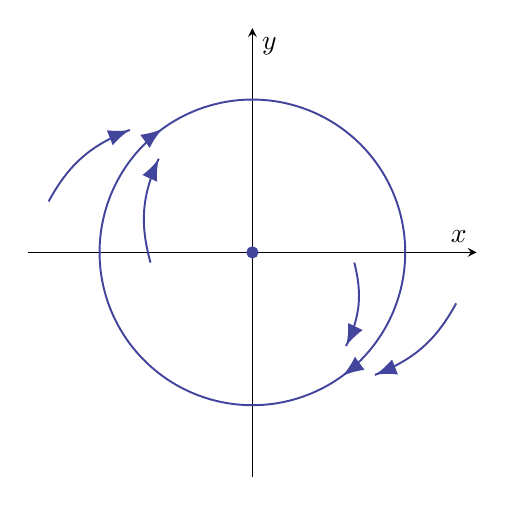
\begin{tikzpicture}[
			lin/.style={
				line width=0.7pt, solid, mark=none,color5
			},		]
		    \begin{axis}[
		    % restrict x to domain=0:360, 
		    restrict y to domain=-2:2,
			% grid=both,
			% scale=1.5,
				% xmode=log,
			% grid style={line width=.1pt, draw=gray!10},
			% major grid style={line width=.2pt,draw=gray!50},
			axis lines=middle,
			ticks=none,
			% minor tick num=5,
			% xmin=1000, 
			% axis lines=none,
			% xmin=-0.2,
			% ymin=-0.2,
			xmax=2.2,
			xmin=-2.2,
			ymin=-2.2,
			ymax=2.2,
			xlabel={$x$},
			ylabel={$y$},
			% rotate=90, 
			lin/.style={
				line width=0.7pt, solid, mark=none,black
			},	
			unit vector ratio*=1 1,		
		]

		  \addplot[
		  	% anchor=origin, % Same as before
            rotate around={90:(0,0)},
		  	data cs=polar,
            % rotate=90,
		  	red,
		  	domain=0:360,
		  	samples=360,
		  	lin,
		  	color5,
		  	% smooth,
		  	decoration={
		  		% post length=1mm,
                % pre length=1mm,
		  		markings,
				mark=at position 0.1 with {\arrow[scale=-1.5, thick]{latex};},
				mark=at position 0.6 with {\arrow[scale=-1.5, thick]{latex};},
				% mark=at position 0.31 with {\arrow{<};},
				% mark=at position 0.51 with {\arrow{>};},
				% mark=at position 0.71 with {\arrow{>};},
				% mark=at position 0.9 with {\arrow{<};}
			},
            postaction={decorate},		 
			] (x,{1.5});

			\draw[fill=color5, color5] (0,0) circle (2pt);
			\draw[lin,decoration={markings,mark=at position 0 with {\arrow[scale=-1.5, rotate=-0,thick]{latex};},},            postaction={decorate}] (45+90:1.3) to[bend left=-20] (axis cs: -1,-0.1);
			\draw[lin,decoration={markings,mark=at position 0 with {\arrow[scale=-1.5, rotate=-0,thick]{latex};},},            postaction={decorate}] (45+90:1.7) to[bend left=-20] (axis cs: -2,0.5);

			\draw[lin,decoration={markings,mark=at position 0 with {\arrow[scale=-1.5, rotate=-0,thick]{latex};},},            postaction={decorate}] (45-90:1.3) to[bend left=-20] (axis cs: 1,-0.1);
			\draw[lin,decoration={markings,mark=at position 0 with {\arrow[scale=-1.5, rotate=-0,thick]{latex};},},            postaction={decorate}] (45-90:1.7) to[bend left=-20] (axis cs: 2,-0.5);			

		% \addplot[domain=0:2.5*pi,samples=100,blue,dec]{-sin(deg(x))} node [right,pos=0.9]{$f(y)$};		  
		    \end{axis}
		\end{tikzpicture}	
\end{document}